% Serenity: suport teoretic. Problema celor n corpuri, cu exemplele Pamant--Luna (n = 2) si Sistemul Solar (n = 6).
% Compilare: pdflatex doua-corpuri.tex (de doua ori, pentru trimiteri)
\documentclass[11pt,a4paper]{article}
\usepackage[T1]{fontenc}
\usepackage[utf8]{inputenc}
\usepackage{amsmath,amssymb,amsthm}
\usepackage[margin=2.5cm]{geometry}
\usepackage{hyperref}
% fara metadate in PDF (data, versiunea pdfTeX, ID)
\pdfinfoomitdate=1
\pdftrailerid{}
\pdfsuppressptexinfo=-1
\hypersetup{pdfcreator={}, pdfproducer={}, pdfauthor={}, pdftitle={}, pdfsubject={}, pdfkeywords={}}
\usepackage{enumitem}
\usepackage{booktabs}
\usepackage{float}
\usepackage[font=small,labelfont=bf]{caption}
\captionsetup[figure]{name=Figura}
\captionsetup[table]{name=Tabelul}
\usepackage{tikz}
\usetikzlibrary{arrows.meta,calc}
\setlength{\emergencystretch}{2em} % evita randurile prea lungi (fara despartire in silabe pentru romana)

% Culori comune pentru desene
\definecolor{corp1}{RGB}{40,110,200}
\definecolor{corp2}{RGB}{150,150,150}
\definecolor{vecr}{RGB}{200,40,40}
\definecolor{forta}{RGB}{180,40,160}
\definecolor{viteza}{RGB}{30,140,60}
\definecolor{cmcol}{RGB}{90,90,90}
\tikzset{
  vec/.style={-{Stealth[length=2.6mm]}, thick},
  axa/.style={-{Stealth[length=2mm]}, gray!70!black},
  ghid/.style={dashed, gray!60},
  corpA/.style={circle, fill=corp1, draw=corp1!60!black, minimum size=7mm, inner sep=0},
  corpB/.style={circle, fill=corp2, draw=corp2!60!black, minimum size=3.6mm, inner sep=0},
}

\newcommand{\vr}{\vec r}
\newcommand{\vv}{\vec v}
\newcommand{\va}{\vec a}
\newcommand{\vR}{\vec R}
\newcommand{\vV}{\vec V}
% derivate in raport cu timpul
\newcommand{\od}[1]{\frac{d #1}{d t}}
\newcommand{\odd}[1]{\frac{d^{2} #1}{d t^{2}}}

\title{Problema celor $n$ corpuri:\\ de la sistemul Pământ--Lună la Sistemul Solar}
\author{Cristian-Lucian Mocanu}
\date{Octombrie 2026}

\begin{document}
\maketitle

\section*{Notă privind redactarea}
Codul \LaTeX{} al acestui document a fost scris integral de Claude, un model de inteligență artificială dezvoltat de Anthropic (\texttt{claude-opus-5-5}). Conținutul a trecut prin modificări succesive, făcute pe baza observațiilor autorului: structura, nivelul de rigoare, notațiile și terminologia au fost stabilite de autor, care a verificat și a aprobat fiecare versiune.

\textbf{Autorul a citit documentul de foarte multe ori, de la cap la coadă, și nu a lăsat în el nicio formulă, niciun pas de calcul și nicio afirmație pe care să nu le înțeleagă.} A cerut explicații și reformulări până când fiecare rând a devenit clar pentru el.

\section*{Scop}
Acest document este suportul teoretic pentru \textbf{Serenity}, un accelerator hardware pentru calculul forțelor gravitaționale în simulări de tip $n$ corpuri. Formulăm problema generală, o particularizăm pentru $n = 2$ și arătăm cum devine un calcul numeric. Încheiem cu două exemple de simulare: sistemul Pământ--Lună ($n = 2$), pentru care cunoaștem mișcarea exactă, și o parte din Sistemul Solar ($n = 6$).

Modelul din Secțiunea~\ref{sec:model} este o idealizare a realității. În interiorul lui nu facem aproximații. Ele apar doar în trei locuri, numite explicit: pasul de timp al calculului numeric (Secțiunea~\ref{sec:numeric}) și constantele și condițiile inițiale din cele două exemple (Secțiunile~\ref{sec:exemplu} și~\ref{sec:solar}).

\section{Modelul}\label{sec:model}
\begin{enumerate}[label=(I\arabic*)]
  \item Sistemul este format din $n$ \emph{puncte materiale}, unde $n \in \mathbb{N}$, $n \ge 2$. Corpurile sunt numerotate cu indicele $i \in \{1, 2, \dots, n\}$: fiecare valoare a lui $i$ desemnează unul și același corp modelat pe toată durata problemei (de exemplu, în Secțiunea~\ref{sec:exemplu}, $i = 1$ este Pământul, iar $i = 2$ este Luna). Corpul $i$ are masa $m_i$ și poziția $\vr_i(t)$, măsurată față de un sistem de referință inerțial.

  (În cod, corpurile sunt numerotate de la $0$ la $n - 1$. Este convenția limbajului C: indicele unui element dintr-un tablou este deplasamentul lui față de începutul tabloului, adică \texttt{bodies[i]} înseamnă \texttt{*(bodies + i)}, deci primul element are indicele $0$.)
  \item Singura interacțiune dintre corpuri este atracția gravitațională, descrisă de legea atracției universale enunțată de Newton, între fiecare pereche de corpuri. Sistemul este izolat: nu există forțe externe.
  \item Corpurile nu se ciocnesc: $\vr_i(t) \neq \vr_j(t)$ pentru orice $i \neq j$ și la orice moment $t$ din intervalul de timp considerat.
\end{enumerate}

\section{Problema celor $n$ corpuri}\label{sec:N}

\subsection*{Ecuațiile de mișcare}
Pentru $i, j \in \{1, \dots, n\}$, $j \neq i$, notăm vectorul care pleacă din corpul $i$ spre corpul $j$ și distanța dintre cele două corpuri:
\[
  \vr_{ij} := \vr_j - \vr_i, \qquad r_{ij} := |\vr_{ij}| .
\]
Cei doi indici îi deosebesc de vectorii de poziție $\vr_i$, care au unul singur. Din definiție, $\vr_{ji} = -\vr_{ij}$ și $r_{ji} = r_{ij}$, iar din (I3), $r_{ij} > 0$.

Conform legii atracției universale, forța exercitată de corpul $j$ asupra corpului $i$ este
\begin{equation}
  \vec F_{j\to i} = G\,\frac{m_i m_j}{r_{ij}^{3}}\,\vr_{ij}, \label{eq:forta}
\end{equation}
unde $G$ este constanta atracției universale. Modulul ei este $G m_i m_j / r_{ij}^2$, direcția este cea a dreptei care unește cele două corpuri, iar sensul este de la $i$ spre $j$ (atracție).

Aplicând principiul al II-lea al mecanicii fiecărui corp și împărțind la $m_i$ obținem, pentru fiecare $i \in \{1, \dots, n\}$:
\begin{equation}
  \boxed{\;\odd{\vr_i} = \sum_{\substack{j=1\\ j\neq i}}^{n} G\,m_j\,\frac{\vr_{ij}}{r_{ij}^{3}}\;} \label{eq:N}
\end{equation}
Accelerația corpului $i$ nu depinde de propria lui masă, ci doar de masele și pozițiile celorlalte corpuri. Nu depinde nici de viteze.

\paragraph{Faptul acceptat (F).} Dacă știm pozițiile și vitezele tuturor corpurilor la momentul inițial, mișcarea lor ulterioară este complet determinată de \eqref{eq:N}. Pe acest fapt se bazează simularea pas cu pas. El are și o consecință practică, pe care o folosim de două ori în document: \emph{dacă găsim, pe orice cale, o mișcare care satisface \eqref{eq:N} la orice moment și pornește din condițiile inițiale date, atunci ea este mișcarea.}

\subsection*{Mișcarea în plan}
În tot documentul lucrăm în planul $xOy$: alegem toate pozițiile și vitezele inițiale în acest plan. Atunci corpurile rămân în plan pentru totdeauna. Într-adevăr, considerăm mișcarea în care corpurile nu părăsesc planul: în ea, toți vectorii $\vr_{ij}$ sunt în plan, deci și accelerațiile date de \eqref{eq:N}; nimic nu împinge vreun corp în afara planului, iar vitezele inițiale nu au componentă în afara lui. O astfel de mișcare satisface \eqref{eq:N} și pornește din condițiile inițiale alese, deci, conform (F), ea este mișcarea. Toți vectorii au așadar două componente, $x$ și $y$.

\subsection*{Ecuațiile pe componente}
Cu $\vr_i = (x_i, y_i)$, notăm diferențele de coordonate dintre corpurile $i$ și $j$:
\[
  \Delta x_{ij} := x_j - x_i, \qquad \Delta y_{ij} := y_j - y_i, \qquad\text{deci}\qquad \vr_{ij} = (\Delta x_{ij}, \Delta y_{ij}), \quad r_{ij} = \sqrt{(\Delta x_{ij})^2 + (\Delta y_{ij})^2}.
\]
Doi vectori sunt egali exact atunci când au componentele egale, deci ecuația vectorială \eqref{eq:N} este echivalentă cu două ecuații scalare, câte una pe fiecare axă:
\begin{equation}
  \odd{x_i} = \sum_{\substack{j=1\\ j\neq i}}^{n} G\,m_j\,\frac{\Delta x_{ij}}{r_{ij}^{3}}, \qquad
  \odd{y_i} = \sum_{\substack{j=1\\ j\neq i}}^{n} G\,m_j\,\frac{\Delta y_{ij}}{r_{ij}^{3}}. \label{eq:comp}
\end{equation}
Aceasta este forma pe care o calculează codul. Distanța $r_{ij}$ este aceeași în ambele ecuații: ea amestecă cele două axe, care altfel ar fi independente.

\subsection*{Legătura cu acceleratorul: de ce $n(n-1)$ termeni}
Pentru orice număr natural $n \ge 3$, ecuațiile \eqref{eq:N} nu au în general o soluție în formă închisă, deci se rezolvă numeric: la fiecare pas de timp se calculează accelerațiile tuturor corpurilor.

Accelerația corpului $i$ este o sumă cu câte un termen pentru fiecare \emph{alt} corp $j$, deci are $n - 1$ termeni. Corpurile sunt $n$, deci în total sunt
\[
  n \cdot (n-1) \text{ termeni de forma } \quad G\,m_j\,\frac{\vr_{ij}}{r_{ij}^{3}}
\]
la fiecare pas de timp. De exemplu, pentru $n = 3$:
\begin{align*}
  \odd{\vr_1} &= \underbrace{G m_2 \tfrac{\vr_{12}}{r_{12}^3}}_{\text{de la 2}} + \underbrace{G m_3 \tfrac{\vr_{13}}{r_{13}^3}}_{\text{de la 3}},\\
  \odd{\vr_2} &= \underbrace{G m_1 \tfrac{\vr_{21}}{r_{21}^3}}_{\text{de la 1}} + \underbrace{G m_3 \tfrac{\vr_{23}}{r_{23}^3}}_{\text{de la 3}},\\
  \odd{\vr_3} &= \underbrace{G m_1 \tfrac{\vr_{31}}{r_{31}^3}}_{\text{de la 1}} + \underbrace{G m_2 \tfrac{\vr_{32}}{r_{32}^3}}_{\text{de la 2}},
\end{align*}
adică $3 \cdot 2 = 6$ termeni (Figura~\ref{fig:termeni}). Pentru $n = 1\,000$ sunt deja $999\,000$ de termeni la fiecare pas. În general,
\[
  n(n-1) \in \Theta(n^2),
\]
adică, pentru $n \ge 2$, numărul de termeni este cuprins între $\tfrac{1}{2}n^2$ și $n^2$: costul unui pas de timp crește pătratic cu numărul de corpuri.

\begin{figure}[H]
\centering
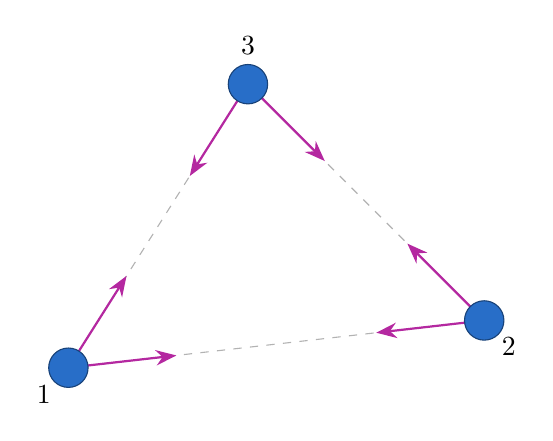
\begin{tikzpicture}[scale=1.2]
  \coordinate (A) at (0,0);
  \coordinate (B) at (4.4,0.5);
  \coordinate (C) at (1.9,3.0);
  \draw[ghid] (A) -- (B) -- (C) -- cycle;
  % cate doua sageti la fiecare corp, spre celelalte doua
  \foreach \X/\Y in {A/B, A/C, B/A, B/C, C/A, C/B}{
    \draw[vec, forta] (\X) -- ($(\X)!1.15cm!(\Y)$);
  }
  \node[corpA, minimum size=5mm] at (A) {};
  \node[corpA, minimum size=5mm] at (B) {};
  \node[corpA, minimum size=5mm] at (C) {};
  \node[below left=1mm] at (A) {$1$};
  \node[below right=1mm] at (B) {$2$};
  \node[above=2.5mm] at (C) {$3$};
\end{tikzpicture}
\caption{Pentru $n = 3$, fiecare corp este atras de celelalte două. Fiecare săgeată este un termen din \eqref{eq:N}: $3$ corpuri $\times$ $2$ termeni $= 6 = n(n-1)$.}
\label{fig:termeni}
\end{figure}

\textbf{Calculul unui astfel de termen pentru o pereche de corpuri este exact operația pe care o implementează Serenity în hardware.} Pipeline-ul primește pozițiile celor două corpuri, $\vr_i$ și $\vr_j$, și masa $m_j$, și produce un termen la fiecare ciclu de ceas. Vitezele nu intră în acest calcul, pentru că membrul drept din \eqref{eq:N} depinde doar de poziții și de mase. Ele intervin abia la avansarea în timp (Secțiunea~\ref{sec:numeric}), care rămâne în software.

\subsection*{Centrul de masă}
Notăm cu $M$ masa totală a sistemului și cu $\vR$ vectorul de poziție al centrului de masă:
\[
  M := \sum_{i=1}^{n} m_i, \qquad \vR := \frac{1}{M}\sum_{i=1}^{n} m_i\,\vr_i .
\]
Înmulțim fiecare ecuație \eqref{eq:N} cu $m_i$ și le adunăm:
\[
  M\,\odd{\vR} = \sum_{i=1}^{n} m_i\,\odd{\vr_i} = \sum_{i=1}^{n}\ \sum_{\substack{j=1\\ j\neq i}}^{n} G\,m_i m_j\,\frac{\vr_{ij}}{r_{ij}^{3}} .
\]
Fiecare pereche de corpuri apare în sumă de două ori: o dată ca $(i, j)$ și o dată ca $(j, i)$. Cei doi termeni sunt
\[
  G\,m_i m_j\,\frac{\vr_{ij}}{r_{ij}^{3}} \qquad\text{și}\qquad G\,m_j m_i\,\frac{\vr_{ji}}{r_{ji}^{3}} = -\,G\,m_i m_j\,\frac{\vr_{ij}}{r_{ij}^{3}},
\]
pentru că $\vr_{ji} = -\vr_{ij}$ și $r_{ji} = r_{ij}$. Ei se anulează doi câte doi (este principiul al III-lea: $\vec F_{j\to i} = -\vec F_{i\to j}$), deci suma este zero și
\[
  \odd{\vR} = \vec 0 .
\]
Așadar, pentru orice $n$, centrul de masă se mișcă rectiliniu uniform: viteza lui, $\vV := \od{\vR}$, este constantă. Cum $M\,\vV = \sum_i m_i \vv_i$, unde $\vv_i := \od{\vr_i}$, centrul de masă este în repaus exact atunci când \emph{impulsul total} $\sum_i m_i \vv_i$ este zero. În particular, dacă la început centrul de masă e în origine și impulsul total e zero, centrul de masă rămâne în origine pentru totdeauna.

\section{Cazul $n = 2$}\label{sec:N2}
Pentru două corpuri, singurul vector relativ care contează este $\vr_{12} = \vr_2 - \vr_1$, iar $\vr_{21} = -\vr_{12}$. Ecuațiile \eqref{eq:N} devin:
\begin{align}
  \odd{\vr_1} &= G\,m_2\,\frac{\vr_{12}}{r_{12}^{3}}, \label{eq:c1}\\
  \odd{\vr_2} &= -\,G\,m_1\,\frac{\vr_{12}}{r_{12}^{3}}. \label{eq:c2}
\end{align}

\begin{figure}[H]
\centering
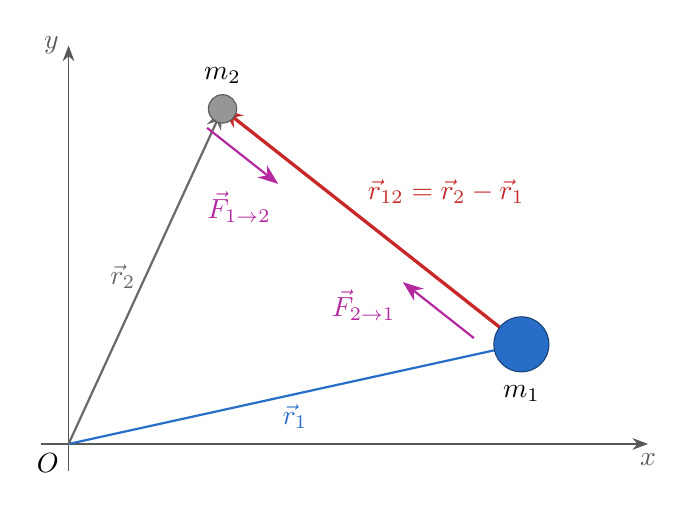
\begin{tikzpicture}[scale=1.15]
  \draw[axa] (-0.3,0) -- (6.4,0) node[below] {$x$};
  \draw[axa] (0,-0.3) -- (0,4.4) node[left] {$y$};
  \node[below left] at (0,0) {$O$};
  \coordinate (A) at (5,1.1);
  \coordinate (B) at (1.7,3.7);
  \draw[vec, corp1] (0,0) -- (A) node[midway, below] {$\vr_1$};
  \draw[vec, corp2!70!black] (0,0) -- (B) node[pos=0.5, left] {$\vr_2$};
  \draw[vec, vecr, line width=1.2pt] (A) -- (B) node[pos=0.55, above right] {$\vr_{12} = \vr_2 - \vr_1$};
  \node[corpA] at (A) {};
  \node[corpB] at (B) {};
  \node[below=4mm] at (A) {$m_1$};
  \node[above=2mm] at (B) {$m_2$};
  \draw[vec, forta] ($(B)+(-0.17,-0.21)$) -- ($($(B)!1.0cm!(A)$)+(-0.17,-0.21)$) node[below left=-1pt] {$\vec F_{1\to 2}$};
  \draw[vec, forta] ($($(A)!0.45cm!(B)$)+(-0.17,-0.21)$) -- ($($(A)!1.45cm!(B)$)+(-0.17,-0.21)$) node[below left=-1pt] {$\vec F_{2\to 1}$};
\end{tikzpicture}
\caption{Două corpuri în planul $xOy$, într-un sistem de referință inerțial cu originea $O$. Vectorul relativ $\vr_{12}$ pleacă din corpul 1 spre corpul 2. Forțele sunt egale în modul, de sensuri contrare ($\vec F_{1\to 2} = -\vec F_{2\to 1}$, conform principiului al III-lea) și pe aceeași direcție, cea a dreptei care unește corpurile. În desen sunt deplasate puțin lateral, ca să nu se suprapună cu $\vr_{12}$.}
\label{fig:inertial}
\end{figure}

\subsection*{Mișcarea relativă}
Scăzând \eqref{eq:c1} din \eqref{eq:c2}:
\begin{equation}
  \odd{\vr_{12}} = \odd{\vr_2} - \odd{\vr_1} = -\,G\,(m_1+m_2)\,\frac{\vr_{12}}{r_{12}^{3}}. \label{eq:rel}
\end{equation}
Vectorul relativ se mișcă deci exact ca un singur corp atras de o masă $m_1 + m_2$ fixată în origine.

\section{De la ecuații la calculul numeric}\label{sec:numeric}

\subsection*{Discretizarea în timp}
Accelerațiile $\va_i$ sunt membrul drept din \eqref{eq:N}. Prin definiție, $\od{\vv} = \lim_{\Delta t\to 0} \frac{\vv(t+\Delta t) - \vv(t)}{\Delta t}$. Calculul numeric înlocuiește limita cu un pas finit $\Delta t$ și avansează sistemul pe momentele $t_k = k\,\Delta t$, cu $k \in \mathbb{N}$:
\begin{equation}
  \vv_i^{\,k+1} = \vv_i^{\,k} + \va_i^{\,k}\,\Delta t, \qquad
  \vr_i^{\,k+1} = \vr_i^{\,k} + \vv_i^{\,k}\,\Delta t, \label{eq:euler}
\end{equation}
unde indicele superior $k$ înseamnă valoarea la momentul $t_k$. Aceasta este metoda Euler explicită.

\textbf{Aceasta este singura aproximație a calculului.} Eroarea ei scade odată cu $\Delta t$ și tinde la zero când $\Delta t \to 0$. La ea se adaugă erorile de rotunjire ale aritmeticii cu precizie finită (\texttt{double} în software, fixed-point în hardware).

Ordinea în care se actualizează vitezele și pozițiile contează mult pe termen lung. Dacă poziția se actualizează cu viteza nouă, $\vv_i^{\,k+1}$, în loc de $\vv_i^{\,k}$, se obține metoda Euler semi-implicită. Comparația dintre cele două metode este studiată separat, în jurnalul proiectului (\texttt{learning/README.md}).

\subsection*{Un pas de calcul}
Cu $\vv_i = (v_{x,i}, v_{y,i})$ și $\va_i = (a_{x,i}, a_{y,i})$, un pas constă în:
\begin{enumerate}
  \item pentru fiecare corp $i$, pornim cu $a_{x,i} = a_{y,i} = 0$ și, pentru fiecare alt corp $j \neq i$:
  \begin{enumerate}[label=(\alph*)]
    \item diferențele de poziție: $\Delta x_{ij} = x_j - x_i$, \; $\Delta y_{ij} = y_j - y_i$;
    \item distanța și factorul comun: $r_{ij} = \sqrt{(\Delta x_{ij})^2 + (\Delta y_{ij})^2}$, \; $s = 1/r_{ij}^3$;
    \item adunăm termenul lui $j$, conform \eqref{eq:comp}: $a_{x,i} \mathrel{+}= G m_j\,s\,\Delta x_{ij}$, \; $a_{y,i} \mathrel{+}= G m_j\,s\,\Delta y_{ij}$;
  \end{enumerate}
  \item actualizarea vitezelor și a pozițiilor tuturor corpurilor, conform \eqref{eq:euler}.
\end{enumerate}
Pașii (a)--(c) sunt calculul pentru o pereche: aceasta este partea pe care o preia acceleratorul. Pasul 2 rămâne în software. În cod, pasul 1 este funcția \texttt{compute\_accelerations}.

Pentru $n = 2$ se regăsesc exact \eqref{eq:c1}--\eqref{eq:c2}: pentru $i = 2$, $j = 1$, diferențele sunt $\Delta x_{21} = -\Delta x_{12}$ și $\Delta y_{21} = -\Delta y_{12}$, deci semnul minus din \eqref{eq:c2} apare singur, fără o formulă separată.

\section{Exemplu: sistemul Pământ--Lună}\label{sec:exemplu}
Corpul $i = 1$ este Pământul, corpul $i = 2$ este Luna.

\subsection*{Constante}
Valorile sunt luate din surse publice (de exemplu, fișele NASA pentru Pământ și Lună):

\begin{table}[H]
\centering
\begin{tabular}{@{}lll@{}}
\toprule
Mărime & Simbol & Valoare \\
\midrule
Constanta atracției universale & $G$ & $6{,}674\times10^{-11}$\,m$^3$\,kg$^{-1}$\,s$^{-2}$ \\
Masa Pământului & $m_1$ & $5{,}972\times10^{24}$\,kg \\
Masa Lunii & $m_2$ & $7{,}342\times10^{22}$\,kg \\
Distanța medie Pământ--Lună & $D$ & $3{,}844\times10^{8}$\,m \\
\bottomrule
\end{tabular}
\caption{Constantele folosite în simulare.}
\label{tab:const}
\end{table}

\subsection*{Aproximațiile exemplului}
\begin{enumerate}[label=(A\arabic*)]
  \item Ignorăm Soarele și restul Sistemului Solar. Pentru Lună, efectul Soarelui nu e neglijabil, deci simularea descrie sistemul de două corpuri Pământ--Lună, nu Luna reală.
  \item Pornim cu o orbită circulară. Orbita reală a Lunii e ușor eliptică ($e \approx 0{,}055$).
  \item Constantele au precizie finită.
\end{enumerate}
Lista conține doar aproximațiile exemplului. Modelul însuși, prin (I1) și (I2), lasă deoparte efecte mai fine, de exemplu forma și rotația corpurilor, mareele sau corecțiile relativiste.

\subsection*{Condițiile inițiale}
Notăm cu indicele $0$ valorile de la momentul inițial $t = 0$: $x_{0i}$ și $y_{0i}$ sunt coordonatele inițiale ale corpului $i$, iar $v_{0i}$ este viteza lui inițială. Alegerile de mai jos sunt cele mai simple care duc la o orbită ușor de verificat:
\begin{itemize}
  \item \textbf{Centrul de masă în origine și în repaus.} Așa rămâne în origine toată simularea (subsecțiunea „Centrul de masă” din Secțiunea~\ref{sec:N}), iar sistemul nu „pleacă” de pe grafic.
  \item \textbf{Ambele corpuri pe axa $x$, de o parte și de alta a originii, la distanța $D$ unul de altul}, deci $y_{01} = y_{02} = 0$ și, la momentul inițial, $r_{12} = D$. Ca centrul de masă să fie în origine ($m_1 x_{01} + m_2 x_{02} = 0$), corpul mai greu stă mai aproape de ea:
  \[
    x_{01} = -\frac{m_2}{M}\,D, \qquad x_{02} = \frac{m_1}{M}\,D .
  \]
  \item \textbf{Vitezele pe axa $y$, de sensuri opuse.} Vrem ca fiecare corp să se rotească pe un cerc în jurul originii. Pe un cerc, viteza e mereu perpendiculară pe rază; raza de start e pe axa $x$, deci viteza inițială are doar componentă pe axa $y$, iar $v_{0i}$ notează această componentă.

  Sensurile opuse nu sunt o alegere: ca centrul de masă să fie în repaus, impulsul total trebuie să fie zero, $m_1 v_{01} + m_2 v_{02} = 0$, deci $v_{01}$ și $v_{02}$ au semne contrare. Cum corpurile sunt de o parte și de alta a originii, asta înseamnă că se rotesc în \emph{același} sens în jurul ei. Alegerea liberă este doar sensul rotației: am ales sensul trigonometric (invers acelor de ceasornic), deci Luna pornește în sensul pozitiv al axei $y$, iar Pământul în sensul negativ. Mărimea vitezelor o calculăm mai jos.
\end{itemize}

\subsection*{Cât de mari trebuie să fie vitezele}
Răspunsul vine din compararea condițiilor impuse de mișcarea circulară cu cele impuse de interacțiunea gravitațională. Facem calculul pentru Lună, apoi pentru Pământ.

\paragraph{Condițiile impuse de mișcarea circulară.} Un corp care se mișcă cu viteza de modul constant $v$ pe un cerc de rază $r_{\text{cerc}}$ își schimbă continuu direcția vitezei. Asta înseamnă că are o accelerație cu direcția razei și sensul mereu spre centrul cercului, de modul
\[
  a_{\text{cerc}} = \frac{v^2}{r_{\text{cerc}}}.
\]
Este un fapt de cinematică (accelerația centripetă) și nu spune nimic despre cauză: fără o astfel de accelerație, corpul s-ar mișca rectiliniu. Cum modulul vitezei nu se schimbă, accelerația nu are componentă de-a lungul vitezei, deci $a_{\text{cerc}}$ este \emph{accelerația totală} a corpului.

\paragraph{Condițiile impuse de interacțiunea gravitațională.} Singura accelerație a Lunii, deci accelerația ei totală, este cea gravitațională, produsă de Pământ. Din \eqref{eq:c2}, modulul ei este
\[
  a_{\text{grav}} = \frac{G m_1}{D^2},
\]
direcția este cea a dreptei Pământ--Lună, iar sensul este spre Pământ.

Pentru mișcarea pe cerc, accelerația totală trebuie să aibă sensul spre centrul cercului pe care se rotește Luna, adică spre centrul de masă (nu spre centrul Lunii: Luna este un punct material). Cele două sensuri coincid: Pământul, centrul de masă și Luna sunt pe aceeași dreaptă, cu centrul de masă între ele, deci a merge de la Lună spre Pământ înseamnă a merge și spre centrul de masă. Direcția și sensul sunt cele corecte, mai trebuie potrivit doar modulul.

\paragraph{Atenție la cele două distanțe.} Raza cercului pe care se rotește Luna este distanța până la \emph{centrul de masă}, $x_{02}$. Gravitația depinde însă de distanța până la \emph{Pământ}, $D$ (Figura~\ref{fig:cerc}). Cele două diferă, pentru că centrul de masă nu e în centrul Pământului.

\begin{figure}[H]
\centering
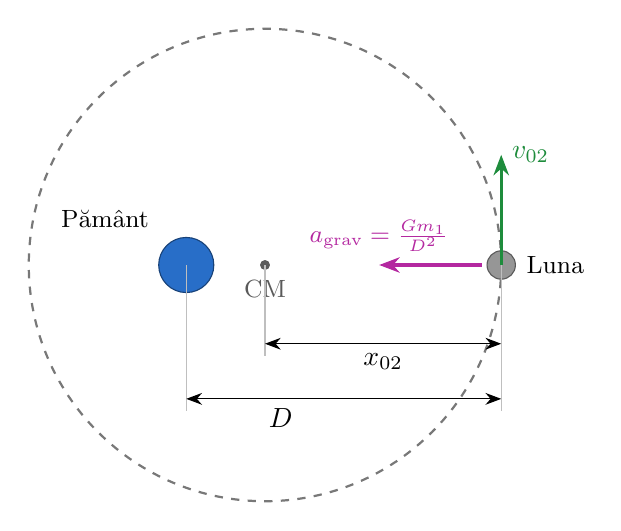
\begin{tikzpicture}[scale=1.0]
  % raport de mase exagerat (3:1)
  \draw[ghid, thick, corp2!80!black] (0,0) circle (3);
  \coordinate (P) at (-1,0);
  \coordinate (L) at (3,0);
  \coordinate (O) at (0,0);
  \node[corpA] at (P) {};
  \node[corpB] at (L) {};
  \fill[cmcol] (O) circle (1.8pt);
  \node[cmcol, below=2pt, font=\small] at (O) {CM};
  \node[above left=3.5mm, font=\small] at (P) {Pământ};
  \node[right=2mm, font=\small] at (L) {Luna};
  % viteza Lunii
  \draw[vec, viteza, line width=1.2pt] (L) -- ++(0,1.4) node[right] {$v_{02}$};
  % acceleratia gravitationala, spre Pamant (si spre centrul cercului)
  \draw[vec, forta, line width=1.2pt] ($(L)+(-0.25,0)$) -- ++(-1.3,0) node[above=1pt, font=\small] {$a_{\text{grav}} = \frac{G m_1}{D^2}$};
  % cote
  \draw[gray!50] (O) -- (0,-1.15); \draw[gray!50] (L) -- (3,-1.85); \draw[gray!50] (P) -- (-1,-1.85);
  \draw[{Stealth[length=2mm]}-{Stealth[length=2mm]}] (0,-1.0) -- (3,-1.0) node[midway, below] {$x_{02}$};
  \draw[{Stealth[length=2mm]}-{Stealth[length=2mm]}] (-1,-1.7) -- (3,-1.7) node[pos=0.3, below] {$D$};
\end{tikzpicture}
\caption{Luna se rotește pe un cerc de rază $x_{02}$ în jurul centrului de masă (CM), dar e atrasă de Pământ, aflat la distanța $D$. Accelerația gravitațională are sensul spre Pământ, deci și spre centrul cercului pe care se rotește Luna. Raportul maselor e exagerat în desen.}
\label{fig:cerc}
\end{figure}

\paragraph{Condiția.} Accelerația totală a Lunii este cea gravitațională; pentru o mișcare circulară uniformă, accelerația totală este cea centripetă. Luna rămâne pe cercul de rază $x_{02}$ exact atunci când cele două sunt egale:
\[
  \frac{v_{02}^2}{x_{02}} = \frac{G m_1}{D^2}.
\]

\paragraph{Calculul.} Înlocuim $x_{02} = \frac{m_1}{M}\,D$:
\[
  v_{02}^2 = \frac{G m_1}{D^2}\cdot\frac{m_1}{M}\,D = \left(\frac{m_1}{M}\right)^{2}\frac{GM}{D}
  \quad\Longrightarrow\quad
  v_{02} = \frac{m_1}{M}\sqrt{\frac{GM}{D}} .
\]
Pentru Pământ, raționamentul e identic: cercul lui are raza $|x_{01}| = \frac{m_2}{M}\,D$, iar accelerația produsă de Lună are modulul $\frac{G m_2}{D^2}$. Rezultă aceeași formulă, cu $m_2$ în loc de $m_1$ și cu semn minus, pentru că Pământul pornește în sensul negativ al axei $y$:
\[
  v_{01} = -\frac{m_2}{M}\sqrt{\frac{GM}{D}} .
\]
Se verifică imediat că $m_1 v_{01} + m_2 v_{02} = 0$, deci centrul de masă stă într-adevăr pe loc.

\paragraph{De ce mișcarea rămâne circulară și uniformă.} Calculul de mai sus verifică potrivirea dintre cele două accelerații doar la momentul inițial. Considerăm următoarea mișcare candidată: Luna parcurge uniform cercul de rază $x_{02}$, iar Pământul cercul de rază $|x_{01}|$, ambele în sens trigonometric. Cele două perioade sunt egale,
\[
  \frac{2\pi x_{02}}{v_{02}} = \frac{2\pi |x_{01}|}{|v_{01}|} = 2\pi\sqrt{\frac{D^3}{GM}},
\]
iar la $t = 0$ corpurile sunt de o parte și de alta a originii. Cum se rotesc la fel de repede, ele rămân la orice moment de o parte și de alta a originii, pe aceeași dreaptă cu ea. De aceea distanța dintre ele nu se schimbă: este mereu $|x_{01}| + x_{02} = D$. La orice moment se repetă deci situația de la $t = 0$, doar rotită în jurul originii, iar calculul de mai sus rămâne valabil. Mișcarea candidată satisface \eqref{eq:c1}--\eqref{eq:c2} la orice moment și pornește din condițiile inițiale alese, deci, conform faptului acceptat (F), ea \emph{este} mișcarea. Așadar orbitele sunt cercuri, iar vitezele au modul constant.

\paragraph{Pe scurt.} Condițiile inițiale ale simulării Pământ--Lună sunt
\[
  x_{01} = -\frac{m_2}{M}\,D, \quad y_{01} = 0, \quad v_{01} = -\frac{m_2}{M}\sqrt{\frac{GM}{D}};
  \qquad
  x_{02} = \frac{m_1}{M}\,D, \quad y_{02} = 0, \quad v_{02} = \frac{m_1}{M}\sqrt{\frac{GM}{D}},
\]
unde $M = m_1 + m_2$.

Cu valorile din Tabelul~\ref{tab:const} obținem valorile de mai jos, date cu suficiente cifre ca să poată fi copiate direct în cod:

\begin{table}[H]
\centering
\begin{tabular}{@{}lrrr@{}}
\toprule
Corp $i$ & $x_{0i}$ (m) & $y_{0i}$ (m) & $v_{0i}$ (m/s) \\
\midrule
1 (Pământ) & $-4\,668\,434{,}6$ & $0$ & $-12{,}442\,354$ \\
2 (Luna)   & $379\,731\,565{,}4$ & $0$ & $1\,012{,}063\,987$ \\
\bottomrule
\end{tabular}
\caption{Condițiile inițiale ale simulării Pământ--Lună. Vitezele inițiale sunt orientate de-a lungul axei $y$: $v_{0i}$ este componenta lor pe această axă, iar componenta pe axa $x$ este $0$.}
\label{tab:ci}
\end{table}

\begin{figure}[H]
\centering
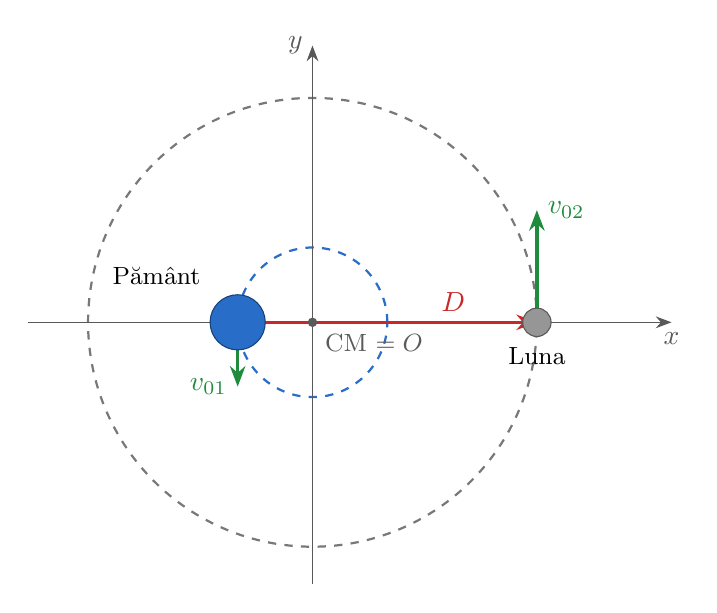
\begin{tikzpicture}[scale=0.95]
  % raport de mase exagerat (3:1), ca sa se vada orbita Pamantului
  \draw[ghid, thick, corp2!80!black] (0,0) circle (3);
  \draw[ghid, thick, corp1] (0,0) circle (1);
  \draw[axa] (-3.8,0) -- (4.8,0) node[below] {$x$};
  \draw[axa] (0,-3.5) -- (0,3.7) node[left] {$y$};
  \coordinate (P) at (-1,0);
  \coordinate (L) at (3,0);
  \draw[vec, vecr, line width=1.1pt] (P) -- (L) node[pos=0.72, above] {$D$};
  \draw[vec, viteza, line width=1.2pt] (L) -- ++(0,1.5) node[right] {$v_{02}$};
  \draw[vec, viteza, line width=1.2pt] ($(P)+(0,-0.36)$) -- ++(0,-0.5) node[left] {$v_{01}$};
  \node[corpA] at (P) {};
  \node[corpB] at (L) {};
  \node[above left=3.5mm, font=\small] at (P) {Pământ};
  \node[below=2mm, font=\small] at (L) {Luna};
  \fill[cmcol] (0,0) circle (1.8pt);
  \node[cmcol, below right=1pt, font=\small] at (0,0) {CM $=O$};
\end{tikzpicture}
\caption{Condițiile inițiale. Ambele corpuri pornesc pe axa $x$, de o parte și de alta a centrului de masă, cu viteze pe axa $y$, de sensuri opuse; apoi se rotesc pe cercuri în jurul originii, în același sens. Raportul maselor e mult exagerat în desen ($3{:}1$ în loc de aproximativ $81{:}1$).}
\label{fig:ci}
\end{figure}

\subsection*{Ce trebuie să obținem}
Pentru aceste condiții inițiale cunoaștem mișcarea exactă a modelului. Orice abatere a simulării de la ea vine din pasul de timp și din rotunjiri:
\begin{itemize}
  \item distanța dintre corpuri rămâne $D = 384\,400$\,km;
  \item centrul de masă rămâne în origine;
  \item Pământul descrie un cerc de rază $\approx 4\,668$\,km în jurul originii (mai mică decât raza Pământului, deci centrul de masă e în interiorul lui), iar Luna un cerc de rază $\approx 379\,732$\,km;
  \item perioada mișcării, adică timpul unei rotații complete, este
  \[
    T = \frac{2\pi x_{02}}{v_{02}} = 2\pi\sqrt{\frac{D^3}{GM}} \approx 2{,}3575\times10^{6}\ \text{s} \approx 27{,}29 \text{ zile}.
  \]
\end{itemize}
Pentru comparație, Luna reală face o rotație completă în jurul Pământului în $27{,}32$ zile. Aceasta se numește \emph{perioada siderală}: timpul după care Luna revine în aceeași poziție față de un sistem de referință inerțial, în practică față de stelele îndepărtate, care par fixe pe cer. Este exact perioada pe care o măsoară simularea, unde axele $x$ și $y$ sunt fixe.

Ea diferă de intervalul de $29{,}53$ zile dintre două faze identice ale Lunii, de exemplu de la o Lună plină la următoarea. Faza depinde de poziția Lunii față de Soare: Luna plină apare când Luna este de partea opusă Soarelui față de Pământ. În cele $27{,}32$ de zile, Pământul a parcurs aproximativ o treisprezecime din orbita lui în jurul Soarelui, deci direcția spre Soare s-a rotit și ea. Luna mai are nevoie de aproximativ două zile ca să ajungă din nou de partea opusă Soarelui. Diferența dintre $27{,}29$ și $27{,}32$ zile vine din aproximațiile (A1) și (A2).

\subsection*{Câți pași are o rotație}
Simularea avansează în pași de durată $\Delta t$, deci numărul de pași dintr-o rotație completă este
\[
  \frac{T}{\Delta t} = \frac{2{,}3575\times10^{6}\ \text{s}}{60\ \text{s}} \approx 39\,291{,}4
\]
pentru $\Delta t = 60$\,s. Cum numărul de pași trebuie să fie natural, după $39\,291$ de pași Lunii îi mai lipsesc aproximativ $0{,}4$ pași până la punctul de start, adică la aproximativ $0{,}4 \cdot 60\ \text{s} \cdot 1\,012\ \text{m/s} \approx 24$\,km de el. Această diferență nu este o eroare a calculului, ci o consecință a faptului că perioada nu este un multiplu întreg al pasului de timp.

\section{Exemplu: Sistemul Solar}\label{sec:solar}
Al doilea exemplu folosește aceleași ecuații, aceeași discretizare și același cod, cu $n = 6$: Soarele și planetele Mercur, Venus, Pământ, Marte și Jupiter. Planetele interioare dau patru orbite apropiate, ușor de urmărit pe același grafic. Jupiter are o masă de peste două ori mai mare decât toate celelalte planete la un loc și este principalul motiv pentru care Soarele se mișcă. Saturn, Uranus și Neptun ar mări desenul de până la șase ori, iar orbitele interioare s-ar strânge într-un punct; adăugarea oricăreia dintre ele înseamnă doar un rând în plus în Tabelul~\ref{tab:solar}.

Corpurile sunt numerotate cu $i = 1$ pentru Soare și $i = 2, \dots, 6$ pentru planete, în ordinea distanței față de Soare.

\subsection*{Constante}
Valorile sunt luate din fișele NASA pentru Soare și pentru planete (\emph{Planetary Fact Sheet}). Constanta $G$ este cea din Tabelul~\ref{tab:const}. Pentru fiecare planetă, $a_i$ este distanța medie față de Soare (semiaxa mare a orbitei reale).

\begin{table}[H]
\centering
\begin{tabular}{@{}llrrr@{}}
\toprule
$i$ & Corp & Masa $m_i$ (kg) & $a_i$ (m) & Perioada reală (zile) \\
\midrule
1 & Soarele & $1{,}989\times10^{30}$ & -- & -- \\
2 & Mercur  & $3{,}301\times10^{23}$ & $5{,}791\times10^{10}$ & $87{,}97$ \\
3 & Venus   & $4{,}867\times10^{24}$ & $1{,}082\times10^{11}$ & $224{,}70$ \\
4 & Pământ  & $5{,}972\times10^{24}$ & $1{,}496\times10^{11}$ & $365{,}26$ \\
5 & Marte   & $6{,}417\times10^{23}$ & $2{,}279\times10^{11}$ & $686{,}98$ \\
6 & Jupiter & $1{,}898\times10^{27}$ & $7{,}785\times10^{11}$ & $4\,332{,}59$ \\
\bottomrule
\end{tabular}
\caption{Constantele pentru Sistemul Solar. Perioadele reale sunt cele siderale și servesc doar la comparație.}
\label{tab:solar}
\end{table}

\subsection*{Aproximațiile exemplului}
\begin{enumerate}[label=(S\arabic*)]
  \item Ignorăm Saturn, Uranus, Neptun, asteroizii și sateliții planetelor. În particular, Pământul este un singur punct material, fără Lună.
  \item Orbitele reale sunt ușor eliptice; cele mai turtite sunt ale lui Mercur ($e \approx 0{,}206$) și Marte ($e \approx 0{,}093$). Noi alegem vitezele inițiale ca și cum fiecare planetă ar fi singură cu Soarele: pentru o astfel de pereche, orbita ar fi exact un cerc de rază $a_i$ (Secțiunea~\ref{sec:exemplu}).

  Cu celelalte planete prezente, orbitele nu mai sunt exact cercuri, dar rămân apropiate de ele, pentru că Soarele este mult mai greu decât orice planetă: cea mai grea, Jupiter, are mai puțin de o miime din masa lui.
  \item Toate orbitele sunt în același plan. Orbitele reale sunt înclinate unele față de altele cu câteva grade (Mercur, cu aproximativ $7^\circ$).
  \item Toate planetele pornesc aliniate, pe axa $x$. Alegerea schimbă doar locul de pe orbită de unde pornește fiecare planetă, nu forma orbitelor.
  \item Constantele au precizie finită.
\end{enumerate}

\subsection*{Condițiile inițiale}
Facem aceleași alegeri ca la Pământ--Lună, cu aceleași notații:
\begin{itemize}
  \item \textbf{Centrul de masă în origine și în repaus.} Așa rămâne în origine toată simularea (subsecțiunea „Centrul de masă” din Secțiunea~\ref{sec:N}).
  \item \textbf{Toate corpurile pe axa $x$}, deci $y_{0i} = 0$. Soarele este în $x_{01}$, iar fiecare planetă $i$ este la distanța $a_i$ de el, în dreapta lui:
  \[
    x_{0i} = x_{01} + a_i, \qquad i = 2, \dots, 6 .
  \]
  \item \textbf{Toate vitezele pe axa $y$}, iar $v_{0i}$ notează componenta lor pe această axă. Planetele pornesc toate în sensul pozitiv al axei $y$, deci se rotesc în sens trigonometric. Acest lucru se întâmplă și în realitate: toate planetele se rotesc în același sens în jurul Soarelui, moștenit de la discul de gaz și praf din care s-a format Sistemul Solar.
\end{itemize}
Necunoscutele sunt deci poziția Soarelui, $x_{01}$, și cele șase viteze.

\paragraph{Poziția Soarelui.} Notăm cu $M = m_1 + m_2 + \dots + m_6$ masa totală. Centrul de masă este în origine exact atunci când $\sum_{i=1}^{6} m_i x_{0i} = 0$. Înlocuim $x_{0i} = x_{01} + a_i$ pentru planete:
\[
  m_1 x_{01} + \sum_{i=2}^{6} m_i\,(x_{01} + a_i) = 0
  \quad\Longleftrightarrow\quad
  M\,x_{01} + \sum_{i=2}^{6} m_i a_i = 0
  \quad\Longleftrightarrow\quad
  \boxed{\;x_{01} = -\frac{1}{M}\sum_{i=2}^{6} m_i a_i\;}
\]
Soarele stă deci puțin la stânga originii: ca la Pământ--Lună, corpul cel mai greu este cel mai aproape de centrul de masă.

\subsection*{Cât de mari trebuie să fie vitezele}
Pentru ca planeta $i$ să se rotească pe un cerc în jurul Soarelui contează doar viteza ei \emph{față de Soare}, adică diferența $v_{0i} - v_{01}$. Dacă am adăuga aceeași viteză ambelor corpuri, distanța dintre ele și accelerațiile ar rămâne aceleași, iar perechea doar ar aluneca uniform: orbita planetei în jurul Soarelui nu s-ar schimba.

Diferența potrivită o luăm din Secțiunea~\ref{sec:exemplu}, cu Soarele în locul Pământului, planeta $i$ în locul Lunii și $a_i$ în locul lui $D$. Scăzând cele două viteze de acolo:
\[
  v_{0i} - v_{01} = \frac{m_1}{m_1 + m_i}\,w_i + \frac{m_i}{m_1 + m_i}\,w_i = w_i, \qquad w_i := \sqrt{\frac{G\,(m_1 + m_i)}{a_i}}, \qquad i = 2, \dots, 6 .
\]
Conform (S2), impunem această diferență pentru fiecare planetă, ca și cum ar fi singură cu Soarele. Rămâne o singură necunoscută, viteza Soarelui, $v_{01}$.

\paragraph{Viteza Soarelui.} O alegem astfel încât centrul de masă al întregului sistem să stea pe loc, adică impulsul total să fie zero, $\sum_{i=1}^{6} m_i v_{0i} = 0$. Calculul este identic cu cel pentru poziția Soarelui, cu $w_i$ în locul lui $a_i$:
\[
  m_1 v_{01} + \sum_{i=2}^{6} m_i\,(v_{01} + w_i) = 0
  \quad\Longleftrightarrow\quad
  \boxed{\;v_{01} = -\frac{1}{M}\sum_{i=2}^{6} m_i w_i\;}
\]
apoi $v_{0i} = v_{01} + w_i$ pentru planete. Soarele pornește deci încet, în sensul negativ al axei $y$, ca Pământul la Pământ--Lună.

\paragraph{Pe scurt.} Cu $M = m_1 + m_2 + \dots + m_6$, condițiile inițiale ale simulării Sistemului Solar sunt
\begin{align*}
  x_{01} &= -\frac{1}{M}\sum_{i=2}^{6} m_i a_i, & y_{01} &= 0, & v_{01} &= -\frac{1}{M}\sum_{i=2}^{6} m_i w_i,\\
  x_{0i} &= x_{01} + a_i, & y_{0i} &= 0, & v_{0i} &= v_{01} + w_i, \qquad i = 2, \dots, 6,
\end{align*}
unde $w_i = \sqrt{G\,(m_1 + m_i)/a_i}$.

Cu valorile din Tabelul~\ref{tab:solar} obținem valorile de mai jos, date cu suficiente cifre ca să poată fi copiate direct în cod:

\begin{table}[H]
\centering
\begin{tabular}{@{}llrrr@{}}
\toprule
$i$ & Corp & $x_{0i}$ (m) & $y_{0i}$ (m) & $v_{0i}$ (m/s) \\
\midrule
1 & Soarele & $-7{,}429\,660\times10^{8}$  & $0$ & $-12{,}645\,4$ \\
2 & Mercur  & $5{,}716\,703\times10^{10}$  & $0$ & $47\,865{,}106$ \\
3 & Venus   & $1{,}074\,570\times10^{11}$  & $0$ & $35\,013{,}907$ \\
4 & Pământ  & $1{,}488\,570\times10^{11}$  & $0$ & $29\,775{,}629$ \\
5 & Marte   & $2{,}271\,570\times10^{11}$  & $0$ & $24\,121{,}860$ \\
6 & Jupiter & $7{,}777\,570\times10^{11}$  & $0$ & $13\,051{,}719$ \\
\bottomrule
\end{tabular}
\caption{Condițiile inițiale ale simulării Sistemului Solar. Vitezele inițiale sunt orientate de-a lungul axei $y$: $v_{0i}$ este componenta lor pe această axă, iar componenta pe axa $x$ este $0$.}
\label{tab:ci-solar}
\end{table}

\subsection*{Ce trebuie să obținem}
\begin{itemize}
  \item Centrul de masă rămâne în origine.
  \item Fiecare planetă descrie o orbită aproape circulară, de rază $\approx a_i$ în jurul Soarelui, cu perioada aproximativ egală cu
  \[
    T_i = 2\pi\sqrt{\frac{a_i^3}{G\,(m_1 + m_i)}},
  \]
  Este legea a III-a a lui Kepler, în forma dată de Newton: pătratul perioadei este proporțional cu cubul razei orbitei. Pentru orbite circulare, ea este exact formula perioadei $T$ din Secțiunea~\ref{sec:exemplu}, cu $m_1 + m_i$ în locul lui $M$ și $a_i$ în locul lui $D$. Pentru orbitele eliptice reale, unde $a_i$ este semiaxa mare, o acceptăm fără demonstrație. Valorile sunt în Tabelul~\ref{tab:perioade}, foarte aproape de perioadele reale.
  \item Soarele nu stă pe loc, ci descrie o curbă mică în jurul centrului de masă, dominată de atracția lui Jupiter. Pentru perechea Soare--Jupiter singură, distanța de la Soare la centrul lor de masă este
  \[
    \frac{m_6}{m_1 + m_6}\,a_6 \approx 7{,}42\times10^{8}\ \text{m},
  \]
  puțin mai mult decât raza Soarelui ($\approx 6{,}96\times10^{8}$\,m): centrul de masă Soare--Jupiter se află chiar în afara Soarelui. Curba nu este un cerc perfect, pentru că și celelalte planete trag de Soare.
\end{itemize}

\begin{table}[H]
\centering
\begin{tabular}{@{}lrr@{}}
\toprule
Planeta & $T_i$ calculat (zile) & Perioada reală (zile) \\
\midrule
Mercur  & $87{,}96$   & $87{,}97$   \\
Venus   & $224{,}64$  & $224{,}70$  \\
Pământ  & $365{,}22$  & $365{,}26$  \\
Marte   & $686{,}71$  & $686{,}98$  \\
Jupiter & $4\,333{,}48$ & $4\,332{,}59$ \\
\bottomrule
\end{tabular}
\caption{Perioadele așteptate, comparate cu cele reale.}
\label{tab:perioade}
\end{table}

\end{document}
